\documentclass[../../memoria.tex]{subfiles}

\begin{document}

\paragraph{}
El siguiente paso es configurar con dichas credenciales el acceso a la consola de AWS. En este caso, se ha instalado la CLI de AWS \cite{awscli} y se han configurado como acceso las credenciales del usuario terraform en el perfil [personal] mediante el comando \textit{aws configure}:

\begin{figure}[H]
    \centering
    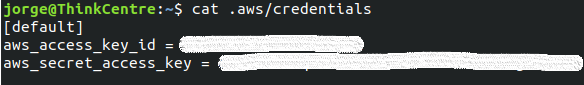
\includegraphics[width=0.7\columnwidth]{figura6.png}
    \caption{Captura del archivo ~.aws/credentials}
    \label{fig:figura6}
\end{figure}

\paragraph{}
Una vez realizada toda esta configuración, se ha creado un repositorio en Github que albergará el código utilizado para la realización de este proyecto. Dicho repositorio será privado y el código que contiene será incluido como anexo en este proyecto.

\paragraph{}
A continuación, se van a explicar partes del código que es interesante mencionar:

\begin{enumerate}
    \item La configuración del \textit{provider}, como se ha mencionado anteriormente, será AWS, se encuentra en las líneas de código que se muestran en la siguiente figura, dentro del archivo que tiene como nombre en el repositorio 00\_main.tf:
          \begin{figure}[H]
              \centering
              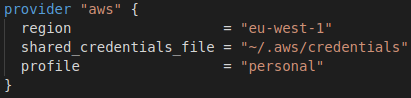
\includegraphics[width=0.7\columnwidth]{figura7.png}
              \caption{Parte del código del fichero 00\_main.tf del repositorio del proyecto}
              \label{fig:figura7}
          \end{figure}
          Como puede observarse en la Figura 7, el \textit{provider} para aws se ha configurado estableciendo la región (eu-west-1) que corresponde a la región de AWS de Irlanda. También se indica el fichero donde se albergan las credenciales de AWS. Dicho fichero es el correspondiente a la Figura 6 y contiene las credenciales del usuario terraform creado anteriormente. La variable \textit{profile} indica que el perfil de dicho archivo de credenciales que se va a utilizar es el llamado personal (el que se puede observar en la Figura 6 como [personal]).

    \item La siguiente parte del código que es interesante mencionar es la referente al \textit{backend}. Esta configuración se muestra en la siguiente imagen:
          \begin{figure}[H]
              \centering
              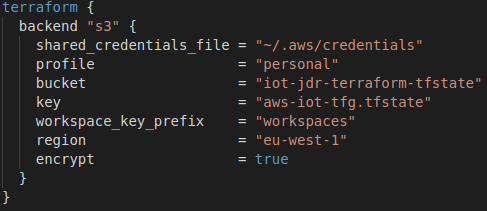
\includegraphics[width=0.7\columnwidth]{figura8.png}
              \caption{Configuración del backend en terraform }
              \label{fig:figura8}
          \end{figure}
          Esta configuración que se puede observar en la Figura 8 es referente al \textit{tfstate} mencionado en el capítulo en el cual se explica Terraform. Por defecto, el \textit{tfstate} se guarda de manera local en el equipo desde el cual se lance la ejecución del comando \textit{terraform apply}. Sin embargo, para este proyecto se ha decidido utilizar un backend remoto que permita guardar dicho \textit{tfstate} en un Bucket S3. Esto permite realizar despliegues desde diferentes equipos recuperando dicho \textit{tfstate}. En este caso se ha decidido guardar encriptado por razones de seguridad y se ha utilizado un \textit{workspace} el cual permite tener diferentes \textit{tfstate} para diferentes entornos de trabajo.

    \item Código de la infraestructura: el resto del código representa la infraestructura y está organizado en:
          \begin{itemize}
              \item Archivos de configuración y variables fijas: 00\_main.tf y 01\_locals.tf: estos archivos configuran el entorno de terraform y contienen variables que son fijas para todo el proyecto.

              \item Archivos de infraestructura del sistema: 02\_elasticsearch.tf y 03\_lambda.tf: estos archivos contienen los recursos de infraestructura que son comunes a todo el sistema. Como bien indican los nombres de dichos archivos, los recursos son Elasticsearch Service y AWS Lambda. Las funciones lambda se guardan en una carpeta separada llamada lambdas y están escritas en Python.

              \item Archivos de infraestructura para una sola tierra de cultivo: 10\_poc\_cropland.tf, 11\_poc\_cropland\_variables.tf y 12\_poc\_cropland\_outputs.tf: contienen la configuración para una tierra de cultivo. La idea es que puedan añadirse tantos archivos similares a estos como tierras de cultivo se desee monitorizar en el mismo sistema, distinguiéndolos por el nombre de la tierra el cual es en este caso poc. El primer archivo contiene los dispositivos IoT, las políticas y roles relacionados con ellos y las funciones lambda que son específicas para una tierra de cultivo. Es interesante mencionar que, para evitar la redundancia de código, se ha elaborado un módulo de terraform para un dispositivo IoT \cite{terraformmodules}. Este módulo se llama aws\_iot\_thing y se puede encontrar en el mismo repositorio.

              \item Archivos de variables y salida del sistema: 99\_variables.tf y 99\_outputs.tf: contienen las variables generales del sistema y la salida pertinente del mismo.

              \item Archivo de variables de entorno: aws-iot-tfg-dev.tfvars: contiene variables de un entorno. Esto está pensado teniendo en cuenta que el mismo código se usará en distintos entornos típicos (desarrollo, preproducción y producción). Esto facilita desarrollos en el sistema sin perder tiempo de servicio del mismo. Este archivo se le pasa a terraform antes de realizar un apply, mediante el uso de la opción -var-file. Cómo se lanza terraform se explicará en el apartado Despliegue de la solución.
          \end{itemize}

\end{enumerate}

\end{document}
